\documentclass[10pt,letterpaper]{article}
\usepackage[margin=1in]{geometry}
\usepackage{amsmath,amssymb,amsthm,booktabs,array,graphicx,url,microtype}
\usepackage{xurl}
\usepackage[hidelinks]{hyperref}
\microtypesetup{protrusion=false}
\newtheorem{theorem}{Theorem}
\newtheorem{proposition}[theorem]{Proposition}
\newtheorem{lemma}[theorem]{Lemma}
\newcommand{\R}{\mathbb R}
\newcommand{\dist}{\operatorname{dist}}
\newcommand{\F}{\mathcal F}
\newcommand{\C}{\mathcal C}
\newcommand{\D}{D^\star}
\newcommand{\ind}{\mathbf 1}
\setlength{\emergencystretch}{2em}
\title{Exact Joint Deformation and Conditional Count Bounds\\ in Ordered Cell Corridors}
\author{Arnav Peram}
\date{}
\begin{document}
\maketitle
\begin{abstract}\normalsize
Segmentation sensitivity in spatial transcriptomics is a joint geometric problem: several transcript reassignments can share a boundary displacement, while individually feasible changes can conflict. We study ordered local cell corridors with heterogeneous Lipschitz limits, thickness bounds, fixed endpoints, boundary bands and pinned structural regions. We prove an ownerwise representation theorem: one polynomial-size rational cut graph preserves the minimum continuous deformation of every feasible transcript assignment, before molecular costs are chosen. The proof combines exact propagation, a simultaneously nearest feasible boundary and analytic integration of excursion layers. Fixed transfer requests admit source-clipped closure under an additional admissibility premise. Hard-budget count spectra follow by target-specific enumeration, with an explicit example separating exact endpoints from all penalty bounds. An exhaustive post-review audit of 42 selected corridors from one Xenium specimen finds 22 of 80 individually feasible baseline transfer pairs jointly infeasible. At area one, marginal thresholds admit 58 pairs but exact joint geometry admits 40. In contrast, all 14,384 conditional single-gene count intervals are exact; a sound marginal enclosure matches every baseline endpoint and fails to be tight in only five enlarged-family rows. The representation therefore establishes exact local geometry without demonstrating routine practical gains for single-gene counts. Certificates identify their corridor and fixed exterior; overlapping corridors define different uncertainty families. The contribution is a constructive continuum-to-assignment reduction with attaining boundaries, evaluated on development data under uncalibrated geometry.
\end{abstract}
\thispagestyle{empty}\hypersetup{pageanchor=false}
\clearpage\setcounter{page}{1}\hypersetup{pageanchor=true}

\section{Joint geometric sensitivity of local transcript assignments}
A segmentation assigns measured molecular coordinates to cells. Shared boundary movement can change several assignments at once; a thickness constraint can prevent individually possible transfers from occurring together. The computational question is to retain these dependencies while minimizing the continuous movement needed to realize each assignment vector. An attaining boundary makes the answer inspectable.

Baysor and Proseg estimate segmentation or assignments \cite{baysor,proseg}; ResolVI models misassignment and related nuisance effects \cite{resolvi}. TISSUE supplies uncertainty-calibrated imputed expression and downstream inference \cite{tissue}. Our object is instead the deterministic function $D^\star(c)$: the least movement realizing a specified assignment $c$ within a declared local geometry. The family and its observation set are part of the question. This distinction is essential when several corridors touch the same cell.

\paragraph{Contribution and prior art.}
We give a constructive ownerwise representation of this continuous cost function. Exact propagation through heterogeneous slope and thickness constraints yields lower and upper envelope families. Their coordinatewise clamp around the source is simultaneously feasible and pointwise nearest. Analytic integration then produces one rational cut graph preserving $D^\star(c)$ for every assignment, before unary molecular costs are specified. The full proof is in Section~\ref{sec:theory}. Hard-budget count bounds and target-specific spectra are consequences of this representation.

Ordered-label and convex-prior cuts \cite{ishikawa,hochbaum}, interacting-surface cuts \cite{li,shah}, and auxiliary-variable reductions \cite{kolmogorov,kohli} provide established machinery. In particular, weighted OR helpers are standard. The result to assess is the exact elimination of the stated coupled continuous geometry, including its ownerwise equality and finite representation size. Lagrangian bounds, enumeration, residual-cut descriptions and conformal ranks are used as standard tools rather than claimed as new general algorithms.

A two-transcript construction shows why individual deformation costs need not determine the joint answer. One boundary with source zero, slope one and clearance $1/20$ must reach height $1/4$ to cross either site $(1/5,1)$ or $(1/5,5/4)$. On $[0,3]$ with zero endpoints and band $[-1/2,1/2]$, each singleton costs $1/16$, while crossing both costs $7/64$. Separating the ordinates to $1$ and $2$ preserves singleton costs and feasibility but makes their joint cost $1/8$. These equal marginals therefore encode different joint functions. Whether that dependence improves a practical query remains an empirical question; our native single-gene census largely favors the simpler enclosure.

\section{The certified object and physical model}
A molecular group \(i\) has one owner \(c_i\) and integer multiplicity \(w_{ig}\) for gene \(g\). A single observed transcript has unit multiplicity. The count in cell \(k\) is
\begin{equation}
 N_{kg}(c)=n^{\rm fixed}_{kg}+\sum_i w_{ig}\ind[c_i=k].\label{eq:count}
\end{equation}
The fixed term is explicit: in the native experiment it includes retained crop observations outside the editable corridor. Undetected molecules and unmeasured genes are outside this count model.

The exact continuous model uses \(m\) ordered boundaries \(f_a(t)\) separating \(m+1\) cells in a local corridor on $I=[t_-,t_+]$. Each boundary has a supplied Lipschitz slope limit, constant band and fixed endpoints. Adjacent boundaries satisfy positive minimum and optional maximum thickness. RNA sites may be points or rectangles with horizontal ownership clearance; nuclear rectangles have immutable owners. All RNA share the same boundary choice. The source \(f^0\) is geometrically admissible. The deformation is
\begin{equation}
 D(f)=\sum_{a=0}^{m-1}\int |f_a(t)-f^0_a(t)|\,dt,
 \qquad \D(c)=\min_{f\in\F(c)}D(f),\label{eq:area}
\end{equation}
with \(\D(c)=+\infty\) for an impossible owner vector. This is summed interface swept area, in square micrometres, not necessarily the tissue area whose owner changes counted once.

At a hard budget \(\delta\), let \(\C_\delta=\{c:\D(c)\leq\delta\}\). A conditional local count query is
\begin{equation}
 L_{kg}(\delta)=\min_{c\in\C_\delta}N_{kg}(c),\qquad
 U_{kg}(\delta)=\max_{c\in\C_\delta}N_{kg}(c).\label{eq:interval}
\end{equation}
An empty uncertainty set is reported explicitly. A certified outer interval may be wider than these exact extrema; the software distinguishes the two. Intermediate integer counts need not all be attainable. Every result is indexed by its corridor, cell identity, gene, geometry, retained observations and budget. The notation should therefore be read as $[L_{kg\mid\mathcal C},U_{kg\mid\mathcal C}]$. These extrema vary only the chosen corridor and fix the exterior. Different corridors can give different intervals for the same cell and gene without a logical conflict: they quantify different families. They cannot be intersected or composed into a whole-cell guarantee merely because their cell identifiers agree.

\paragraph{Threshold obligations.}
Number boundaries $a=0,\ldots,m-1$ and cells $0,\ldots,m$. For a site $i$ in group $g(i)$, define
\begin{equation}
b_{ga}=\ind[c_g\leq a],\qquad b_{ga}\leq b_{g,a+1}.\label{eq:bits}
\end{equation}
A rectangular site $[x_i^-,x_i^+]\times I_i$ and clearance $\rho>0$ impose
\begin{equation}
b_{g(i),a}=1\Rightarrow f_a\geq\ell_i=x_i^++\rho,\qquad
b_{g(i),a}=0\Rightarrow f_a\leq u_i=x_i^--\rho
\quad\text{on }I_i.\label{eq:obligations}
\end{equation}
Let the boundary bands be $[\underline b_a,\overline b_a]$ and gaps be $[d_a^{\min},d_a^{\max}]$, allowing infinite upper gaps. Fixed structural groups use the same obligations with pinned owner bits. A rational piecewise-linear source satisfies the geometric constraints; it need not satisfy every possible site rectangle. For rational unary costs $C_g$ and $\lambda\geq0$, the penalized objective is
\begin{equation}
\min_{f,c}\left\{\lambda D(f)+\sum_g C_g(c_g)\right\}.\label{eq:objective}
\end{equation}
\section{Exact finite elimination of continuous geometry}\label{sec:theory}
\subsection{How a boundary restriction constrains its neighbors}
Create a boundary-index graph with $a\to a+1$ of weight $d_a^{\min}$ and, when finite, $a+1\to a$ of weight $-d_a^{\max}$. Let $\Delta_{ab}$ be its maximum path weight, with $\Delta_{aa}=0$ and $-\infty$ for no path. Source feasibility excludes positive cycles. Max-plus Floyd--Warshall computes $\Delta$ in $O(m^3)$ arithmetic operations. Define
\begin{equation}
 K_{ab}(r)=\max_c\{\Delta_{ac}+\Delta_{cb}-s_c r\},\qquad r\ge0,\label{eq:kernel}
\end{equation}
using only existing paths.

\begin{lemma}[Propagation closure]\label{lem:kernel}
Every admissible family satisfies $f_b(v)\ge f_a(u)+K_{ab}(|u-v|)$. This is the strongest inequality obtained by finite composition of the given longitudinal Lipschitz and same-coordinate separation constraints.
\end{lemma}
\begin{proof}
For each $c$, transfer from $a$ to $c$ at $u$, travel to $v$ on $c$, then transfer to $b$. Conversely, in any composite path choose a surface $c$ of minimum slope among the longitudinal steps. Its vertical steps before and after that visit total at most $\Delta_{ac}+\Delta_{cb}$. Its absolute longitudinal travel is at least $|u-v|$, at rates at least $s_c$. Its implied bound cannot exceed that term of~\eqref{eq:kernel}. Zero longitudinal travel is covered at $r=0$.
\end{proof}
Thus $K_{ab}(0)=\Delta_{ab}$, kernels are nonincreasing, and
\begin{equation}
 K_{ab}(r_1+r_2)\ge K_{ac}(r_1)+K_{cb}(r_2).\label{eq:composition}
\end{equation}
A destination-$b$ term with rate $s_c>s_b$ is dominated by the direct $b$ term, since $\Delta_{ac}+\Delta_{cb}\le\Delta_{ab}$. The corresponding source statement holds as well. These observations ensure the required propagated slopes.



\subsection{Finite constraints for realizable assignments}
For a lower obligation $(a,I_i,\ell_i)$, forbid its activating bit value $1$ if, for any destination $b$ and kernel term $(d,s)$ of $K_{ab}$,
\begin{equation}
 \ell_i+d>\overline b_b\quad\text{or}\quad
 \ell_i+d>f_b^0(e)+s\dist(e,I_i)\quad\text{for }e\in\{t_-,t_+\}.\label{eq:unarylower}
\end{equation}
For an upper obligation $(a,I_i,u_i)$, forbid activating value $0$ if a term $(d,s)$ of $K_{ba}$ satisfies
\begin{equation}
 u_i-d<\underline b_b\quad\text{or}\quad
 f_b^0(e)>u_i-d+s\dist(e,I_i).\label{eq:unaryupper}
\end{equation}
For every ordered lower/upper pair add
\begin{equation}
 b_{g(i),a}\Longrightarrow b_{g(j),b}
 \quad\text{if}\quad \ell_i+K_{ab}(\dist(I_i,I_j))>u_j.\label{eq:implication}
\end{equation}
Same-bit implications are tautologies. Add~\eqref{eq:bits} and pins $b_{ga}=\ind[c_g^{\rm fixed}\le a]$ for all structural groups. Equations~\eqref{eq:unarylower}--\eqref{eq:implication} apply to RNA and pinned structures identically. Contradictory unary fixes or implications mean model infeasibility.

\begin{theorem}[Exact ownership feasibility]\label{thm:feas}
The finite restrictions above characterize exactly the universal-region owner vectors realizable in the declared continuous family.
\end{theorem}
\begin{proof}
Necessity follows from Lemma~\ref{lem:kernel}, using the smallest interval distance for a nonincreasing kernel. For sufficiency, propagate selected lower and upper obligations into envelopes $L_b,U_b$. Their molecular contributions are
\[
 \ell_i+K_{ab}(\dist(t,I_i)),\qquad
 u_j-K_{ba}(\dist(t,I_j)),
\]
respectively. Include fixed endpoints as both lower and upper point data; include bands as interval data across all of $I$. Equation~\eqref{eq:composition}, the triangle inequality, and~\eqref{eq:implication} put every lower contribution below every upper contribution; the unary tests handle their comparisons to fixed data. Hence $L_b\le U_b$. For every directed separation edge $a\to b$ of weight $d$, closure gives $K_{ob}\ge K_{oa}+d$, hence $L_b\ge L_a+d$. Similarly $K_{ao}\ge d+K_{bo}$ implies $U_a\le U_b-d$. Applying this to both directed edges enforces both finite gap bounds, not just the minimum. Dominated rates preserve each surface's Lipschitz bound. Fixed data enforce bands and endpoint equality. Thus the envelopes are feasible realizations. Nesting specifies exactly one cell per group.
\end{proof}
For example, when two boundaries have fixed separation one, slopes two and $1/4$, and fixed source heights zero and one, the left boundary can reach at most $1/8$ at distance $1/2$ from the endpoint. Its own slope alone would give the incorrect limit one. This demonstrates why a neighboring regularity constraint cannot be ignored.

\subsection{A nearest boundary and its integrated cost}
For an owner vector $c$, define
\[
 D^\star(c)=\min_{f\in\mathcal F(c)}D(f),
\]
with $+\infty$ for an empty realization family.
\begin{theorem}[Ownerwise integrated-cost representation]\label{thm:cut}
For rational input, a polynomial-size directed graph $G_D$ with molecular threshold vertices $b(c)$, auxiliary vertices $y$, and hard arcs satisfies:
\begin{enumerate}
\item A hard-feasible cut with molecular labels $b(c)$ exists exactly when $\mathcal F(c)\ne\varnothing$.
\item For \emph{every} such owner vector, before choosing molecular costs,
\begin{equation}
 \min_y\operatorname{Cut}_{G_D}(b(c),y)+\kappa=D^\star(c).\label{eq:ownerwise}
\end{equation}
\end{enumerate}
Here $\kappa$ is an explicitly recorded rational constant, initially zero; geometric capacities are rational and hard arcs are logical constraints. After the unary costs and $\lambda$ are chosen, their finite implementation capacity is set above the sum of all finite capacities. The fixed object is the topology and geometric representation, not a numerical big-$M$ valid for arbitrary future unaries. After common-denominator scaling, divide the integer cut value by that scale. Consequently, for arbitrary rational unary costs and rational $\lambda\ge0$, one finite cut either detects model infeasibility or returns optimal owners and an attaining rational piecewise-linear boundary for~\eqref{eq:objective}.
\end{theorem}
\begin{proof}
For any feasible owner vector, set
\begin{equation}
 f_b^*(t)=\min\{U_b(t),\max\{L_b(t),f_b^0(t)\}\}.\label{eq:clamp}
\end{equation}
Families satisfying lower difference inequalities are closed under componentwise min and max: from $f_b\ge f_a+d$ and $g_b\ge g_a+d$ both operations preserve the inequality. Min/max also preserve scalar Lipschitz bounds, bands, and endpoints. Hence~\eqref{eq:clamp} is feasible. Every realizing boundary lies in $[L_b,U_b]$ pointwise; the clamp is its nearest point to $f_b^0$. It therefore minimizes each absolute displacement and their integrated sum.

A propagated restriction has a tent-shaped profile, called a cone. The upward displacement is a maximum of nonnegative functions
\[
 [\ell_i+d-s\dist(t,I_i)-f_b^0(t)]_+
\]
activated by bits; downward functions are activated by complementary bits. Fixed geometric data already satisfied by $f^0$ cannot push it outward. Selected structural and RNA obligations are retained even when they are not nominal flips: the source need not satisfy every uncertain RNA rectangle. Upward and downward displacement cannot both be positive for feasible owners.

Split $I$ at plateau endpoints, source knots, zeros, and positive pair intersections. On a slab, positive affine heights have fixed order $h_1\ge\cdots\ge h_k>0$, with $h_{k+1}=0$. For activated groups, their maximum is exactly
\begin{equation}
 \sum_{j=1}^k(h_j-h_{j+1})\ind[\text{at least one of the top-$j$ activations holds}].\label{eq:layers}
\end{equation}
Integrate each affine difference rationally. Positive OR layers use a helper $z$, hard arcs $b\Rightarrow z$, and a helper-to-sink capacity. Complement OR layers use $z\Rightarrow b$ and a source-to-helper capacity. Repeated activations are not independent variables. Nested sets share predecessor helpers, giving constant arcs per distinct layer. These are standard higher-order reduction gadgets~\cite{kolmogorov,kohli}; their weights here are exact geometric integrals.

Finally,
\begin{equation}
 C_g(c_g)=C_g(m)+\sum_{a=0}^{m-1}[C_g(a)-C_g(a+1)]b_{ga}.\label{eq:unary}
\end{equation}
Shift negative unaries by a recorded constant and include all feasibility/pin arcs. Before unaries are added, minimization over the OR helpers yields exactly the integrated clamp displacement for each fixed $b(c)$, proving~\eqref{eq:ownerwise}. Adding~\eqref{eq:unary} and $\lambda$ therefore preserves the minimum of~\eqref{eq:objective}. Recover owners and~\eqref{eq:clamp}. Scaling rational capacities by a common denominator permits integer flow/cut proofs; hard capacity one greater than the sum of finite capacities ensures a hard-arc cut occurs only when the pinned model is infeasible.
\end{proof}


\paragraph{Aggregated graph size and encoding.}
Let $N$ count all merged obligation rectangles, including pinned nuclear structures; $G$ counts groups. On boundary $b$ there are $M_b=O(Nm^2)$ propagated cone terms across both polarities and $J_b$ source knots. A direct arrangement can have $Q_b=O(M_b^2+M_bJ_b+J_b+1)$ slabs, but charging every prefix on every slab overcounts the \emph{aggregated graph}.

For one polarity, write the untruncated cone terms as $g_i(t)=\alpha_i-s_i\dist(t,I_i)$. Subtracting or adding a common source does not change their relative order. Each pair of constant-piece affine cones changes order only constantly many times. Resolve simultaneous events into adjacent swaps; each swap changes only one full prefix set. Starting with $M_b$ prefixes therefore yields $O(M_b^2+M_b)$ distinct sets. Positivity selects some of these prefixes, and repeated activation labels cannot increase their count. Retaining zero-weight predecessors as necessary gives a constant-arc helper construction. Thus
\begin{align}
 |V_{\rm cut}|&=O\!\left(Gm+\sum_b(M_b^2+M_b)\right),\nonumber\\
 |E_{\rm cut}|&=O\!\left(Gm+N^2m^2+\sum_b(M_b^2+M_b)\right).\label{eq:size}
\end{align}
The auxiliary-size contribution is $O(N^2m^5)$. This is a representation bound, not a faster implementation claim: the current compiler still scans slab layers before merging. Source knots affect integration work, rational coefficient length, and reconstruction. The supplement treats ties, repeated labels and helper predecessors explicitly.

All rationals are binary encoded. Closure weights use simple paths; intersections, affine integration and sums have polynomial bit complexity. A common capacity denominator has bit length at most the sum of its constituent denominator lengths. Group-set bookkeeping and construction work remain polynomial and can be large. No asymptotic dominance over every compressed height representation follows.

\paragraph{An exact critical-mesh alternative.}
For each boundary, collect every propagated lower/upper obligation piece, fixed geometric piece, and source piece, before choosing owners. A common mesh contains their breakpoints and all same-boundary crossings. On every mesh interval, the canonical clamp for \emph{any} feasible ownership vector selects one affine piece and its displacement has constant sign. Its trapezoidal cost is exact. Conversely, interpolating any feasible nodal vector preserves the linear constraints, and its trapezoidal absolute-displacement cost upper-bounds its integral. Because the canonical minimizer is included, the nodal minimum equals $D^\star(c)$ for every $c$.

Restrict each nodal height to the candidate-function values there. The same canonical minimizer remains available. Ordered height bits encode each choice; slope, thickness and ownership inequalities become implications, and trapezoidal weights are unary nodal costs. This is a second exact surface-cut reduction. The supplement gives the full construction, safe pin-envelope pruning, and a polynomial size bound. It uses absolute displacement; exact trapezoids are not asserted for higher loss powers. The direct graph instead integrates activation layers across intervals and can merge recurring activation sets. Neither construction is claimed to dominate all possible compressed surface representations.

\section{Hard-budget bounds, exact refinement and their limits}
Write an integer-valued query as \(S(c)=a+\sum_i s_i(c_i)\), where \(a\) contains fixed exterior contributions. Counts and fixed rational linear contrasts, after integer scaling, have this form. For each rational \(\mu\geq0\), a cut solves
\[
 m_+(\mu)=\min_{c:\F(c)\ne\varnothing}\{\mu\D(c)-\sum_i s_i(c_i)\},\qquad
 m_-(\mu)=\min_{c:\F(c)\ne\varnothing}\{\mu\D(c)+\sum_i s_i(c_i)\}.
\]
\begin{proposition}[Lagrangian count bounds]
For every \(c\in\C_\delta\),
\begin{equation}
 a+\lceil m_-(\mu)-\mu\delta\rceil
 \ \leq\ S(c)\ \leq\
 a+\lfloor\mu\delta-m_+(\mu)\rfloor.\label{eq:dual}
\end{equation}
The strongest bounds from any finite set of nonnegative multipliers remain valid.
\end{proposition}
\begin{proof}
Optimality of \(m_+\) implies \(\mu\D(c)-\sum_i s_i(c_i)\geq m_+\). Rearrange, use \(\D(c)\leq\delta\) and round down since \(S\) is integer. Apply the same argument to \(-S\) for the lower bound. Each multiplier is individually sound, irrespective of its selection method.
\end{proof}
Every returned boundary is also evaluated directly. A feasible witness supplies attained inner extrema, giving
\[
 L_{\rm bound}\leq\min S\leq L_{\rm witness},\qquad
 U_{\rm witness}\leq\max S\leq U_{\rm bound}.
\]
Only matching endpoints receive status \texttt{exact}; otherwise the result carries its gaps. Rational arithmetic makes the rounding in (\ref{eq:dual}) unambiguous. Model infeasibility and resource limits are distinct outcomes.

\paragraph{A genuine penalty gap.}
Three separated groups of co-located unit transcripts contribute counts \(2,3,3\), with minimum areas \(4,9,9\). At budget 10, the true maximum is 3. Every nonnegative penalty upper bound is at least 4: a mixture of \((D,S)=(4,2)\) with weight \(2/3\) and \((22,8)\) with weight \(1/3\) has expected area 10 and count 4. The multiplier \(\mu=1/3\) attains that bound. Thus additional penalty optimization cannot by itself recover the exact endpoint. Figure~\ref{fig:gap} shows the executed continuous-tent construction.
\begin{figure}[t]
\centering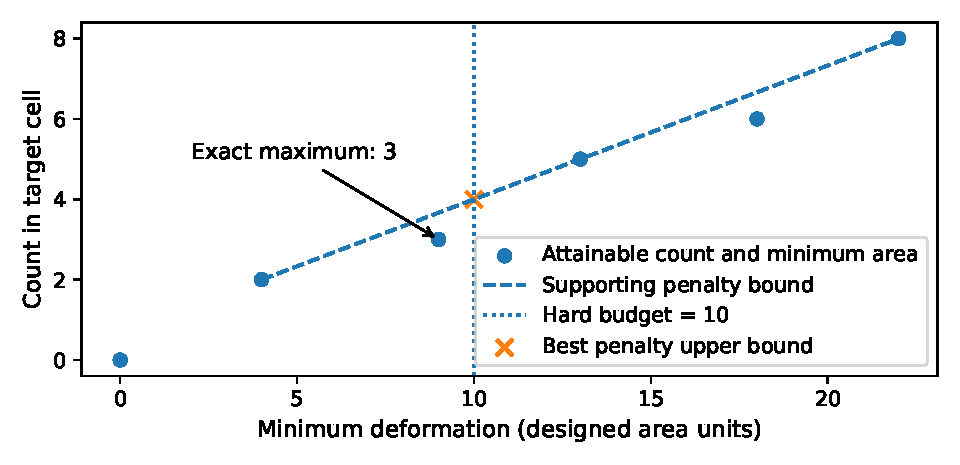
\includegraphics[width=\textwidth]{figures/hard_budget_gap.pdf}
\caption{A designed hard-budget gap. Each point is an attainable count and its minimum area. At area 10, the largest attainable count is 3, whereas the best affine penalty bound is 4. Exact target projection resolves the gap.}\label{fig:gap}
\end{figure}

\subsection{Exact projection onto relevant transcripts}
The source-clipping shortcut requires that the source realizes \emph{every source-owner and structural obligation at zero deformation}. This is stronger than geometric source feasibility and is checked by the implementation. For owner pins, propagate required true threshold bits forward and required false bits backward in the implication graph. A conflict proves infeasibility; otherwise retain source bits where unforced.

This completion is feasible. Every displacement-inducing obligation activated away from the source is forced in every feasible completion; every retained source-active obligation has zero source-relative excursion. Its envelope therefore has no greater movement at any point than another completion. Reconstruction gives the least deformation for the requested pins while leaving collateral molecules free.

\begin{proposition}[Target-specific exact spectrum]
Under the source-admissibility premise, if \(S\) depends on the owners of \(r\) groups, enumerating their feasible owner assignments and applying minimum completion computes
\(d(v)=\min_{S(c)=v}\D(c)\) exactly in
\(O((m+1)^r T_{\rm completion})\) work. Equation~(\ref{eq:interval}) follows by taking the least and greatest \(v\) with \(d(v)\leq\delta\).
\end{proposition}
\begin{proof}
Every feasible complete assignment restricts to one enumerated target assignment. Its minimum completion has the same score and no greater area. Conversely, each accepted completion is a complete feasible assignment attaining its recorded score and area. Minimizing in both directions proves equality.
\end{proof}
The exponent depends on the transcripts that affect the requested statistic, not all collateral RNA. This is still exponential in \(r\), and a capped, incomplete spectrum cannot certify an omitted outcome. Source-inconsistent universal-location models instead use the cut bounds and an explicit minimum-area feasibility check.

The same argument handles joint count vectors and an additional all-RNA reassignment cap. For each target pinning, source clipping also minimizes the total weight of changed owners: every changed group has a forced bit differing from its source. The supplement gives the two-resource bound and its exact-spectrum tests.

\subsection{Joint questions and all optimal assignments}
For a finite set of target genes/cells, store each joint count tuple and its minimum area. A predicate is \texttt{always}, \texttt{never} or \texttt{variable} only after considering all budget-feasible tuples. This supports exact expression-presence conjunctions without multiplying marginal possibilities. A robust expression conjunction alone is not a signaling inference.

For a fixed penalized objective, the residual strongly connected component DAG represents all minimum cuts by forward-closed component sets \cite{picard}. The implementation returns that DAG and marginal owner domains. It does not confuse these optimal assignments with the larger hard-budget family. Standard monotone parametric-flow conditions apply to nonnegative rewards for an extreme cell after scaling \(D-tN\) \cite{gallo}. Middle-cell membership uses two threshold bits with opposite signs; an implemented two-RNA counterexample has nonnested cuts. We use repeated exact cuts rather than claim one parametric flow for every query.

\paragraph{Composition and scope.}
Independent patches admit min-plus composition only after establishing disjoint editable interiors and observations, compatible fixed traces and attachment to fixed connected cell cores. Native overlapping corridors meet no such automatic composition premise. Their union describes ``one of these local interventions''; simultaneous deformations require a separate consistent model. A complete overlap audit finds 19 of 51 cells in multiple corridors (at most seven), with 178 distinct cell/gene/budget/setting keys receiving different local intervals: 74 baseline and 104 enlarged. The software therefore retains family identifiers and separately exports exact union-of-one-corridor bounds. The supplement gives composition, a distance-based raster relaxation and calibration diagnostics. Those additions neither enlarge the exact corridor theorem nor provide biological validation.

\section{Executed evaluation}
\subsection{Exhaustive joint-transfer audit}
Following review of the weak single-gene endpoint results, we evaluated every pair of individually feasible non-source transfers on distinct unit transcripts in each of the same 84 corridor/settings. Pair selection uses no gene panel or outcome filter. This is a post-review exhaustive development audit, not a preregistered external study. Collateral transcripts remain free, so each pair asks for the minimum movement that realizes its two pinned transfers.

\begin{table}[!ht]\centering
\begin{tabular}{lrr}\toprule
Quantity & Baseline & Enlarged\\\midrule
Corridor/settings &42&42\\
Settings containing eligible pairs &8&26\\
Individually feasible moves &48&171\\
Candidate pairs &80&652\\
Jointly infeasible pairs &22&85\\
Feasible pairs with cost above maximum singleton &51&519\\
Feasible pairs with cost below singleton sum &23&144\\\bottomrule
\end{tabular}
\caption{Complete pair census on distinct unit transcripts. Marginal costs can omit joint incompatibility and understate the movement budget; their sum can overstate shared movement. Counts are dependent computational queries.}\label{tab:pairs}
\end{table}

At area $1\,\mu$m$^2$, baseline singleton thresholds admit 58 pairs, while exact joint geometry admits 40; 18 marginal admissions therefore fail the joint budget or constraints. The enlarged family admits 435 by singleton thresholds and 315 exactly, a difference of 120. An additive-cost test retaining joint feasibility admits 39 and 304, respectively: shared movement recovers one baseline and eleven enlarged-family pairs. These comparisons assess requested assignments, not superiority of marginal gene-count endpoints. Only one baseline pair and 22 enlarged-family pairs concern two transcripts of the same gene.

A separate event-compiled cut replay checks all 732 pair results, with exact primal/dual certificates and no discrepancy. Complete budget-grid results and attaining boundaries are retained. The presence of effects in this deliberately joint query motivates retaining the ownerwise function; their frequency in these selected corridors does not establish prevalence in tissue or corrected biological ownership.

\subsection{Complete native count census}
The unchanged development inputs contain 42 selected corridors in two crops from one public Xenium lung specimen \cite{dataset}. They include 464 repeated local records, 387 unique local transcripts and 51 source cells; there are 7,370 retained measured-gene RNA records in the crops. We rechecked every source owner against the masks. Outside each corridor, retained crop counts are fixed. Border-clipped cells are not presented as complete whole-cell expression profiles.

Every locally observed gene is crossed with every cell in its corridor, under both the original baseline and inherited enlarged geometry. The latter extends endpoints and doubles slope/band allowances without adding tissue observations. Eight area budgets are fixed in the protocol. This gives 1,798 cell--gene questions and 14,384 exact intervals. A sparse matrix export also includes 18,096 unchanged positive-count rows; these are algebraic copies rather than additional optimizations. The multiplier set is \(\{0,1/16,1/4,1,4,16,64\}\); 25,172 rational cuts are checked. Target projection considers 2,358 assignments in total, with local gene multiplicity at most 3. All 13 cases not closed by both dual endpoints and attained witnesses are resolved by complete projection. Five of these have loose finite-grid dual endpoints; the remainder need attaining witnesses. Finite-grid looseness is distinct from an irreducible duality gap.

\begin{table}[!ht]
\centering
\begin{tabular}{r rr rr}
\toprule
&\multicolumn{2}{c}{Non-singleton intervals /899}&\multicolumn{2}{c}{Source-zero counts that can become positive}\\
Budget ($\mu$m$^2$)&Baseline&Enlarged&Baseline&Enlarged\\\midrule
0&0&0&0&0\\
0.1&40&72&14&21\\
0.5&68&204&27&72\\
1&80&265&30&92\\
2&92&297&34&100\\
4&94&307&35&102\\\bottomrule
\end{tabular}
\caption{Exact conditional count sensitivity. Each row uses the same 899 cell--gene entries per geometry. Repeated budgets/corridors are dependent queries, not biological replicates.}
\end{table}

A separate native checker uses the older scanning compiler, late owner pins and full target assignment enumeration rather than the new spectrum routine. It reconstructs all 1,798 spectra, checks 14,384 intervals, and replays 1,176 stored root flow proofs, with no disagreement. It shares primitive geometry and ingestion; this is independent-code-path validation, not independent researchers.

\paragraph{A concrete count certificate.}
For PECAM1 in source cell 153124 of corridor 4037abe9fea38e, the observed count is 0. The interval remains $[0,0]$ at area 1 and becomes $[0,1]$ at areas 2 and 4. The latter has an exact attaining boundary, shown in the supplement. The neighboring cell's measured count correspondingly ranges from 0 to 1. This establishes an allowed alternative to an observed count, not biological absence or corrected ownership.


\paragraph{Joint counts and the strong simple baseline.}
In the previously identified three-cell corridor c8f8188430d092, the enlarged model at area 4 gives intervals $[0,1]$ for MDM2 in right cell 153965 and TFPI in left cell 153959. Yet both counts cannot become positive together under the original minimum thickness. Relaxing only that additional minimum permits the joint event. The full joint-count projection verifies the distinction; one propagated inequality already explains this selected obstruction.

We also compare every native interval with a sound marginal envelope formed from individually feasible owners within the same area budget. Joint budgeting tightens only five enlarged-family intervals and none at baseline. An additive singleton-cost inner approximation misses no extrema in this count census. These adverse attribution results remain explicit: most native single-gene questions are easy, and the corpus does not demonstrate a broad computational advantage over individual thresholds.

\subsection{Adversarial checks}
The budget suite compares 4,350 complete owner vectors across 60 models, 183 score minima and 398 hard-budget enclosures; all agree. It explicitly retains the count 3 versus penalty 4 gap. Twenty additional models give 80 exact two-resource spectra and 480 sound two-resource bounds. Joint outcomes and residual optimal-owner domains are checked against exhaustive truth; deliberate model, score and certificate alterations are rejected. All findings, including non-tight intervals and failed applicability premises, are retained in the artifact.

\section{Interpretation and availability}
The graph preserves a continuous assignment-cost function, including shared deformation and coupled feasibility. Count spectra expose both feasible changes and hard-budget exclusions within one specified corridor. On the present native questions, exact joint reasoning rarely tightens the simple marginal enclosure; exact geometry is a computational guarantee rather than evidence of routine empirical superiority. The principal claim is therefore the representation theorem and its inspectable local consequences.

\paragraph{Limitations.}
The native data are selected development corridors from one donor with uncalibrated slope, band and area settings. Most single-gene questions contain one local transcript. Exterior assignments stay fixed, and overlapping corridors define distinct conditional families. The continuum theorem excludes general tessellations, junctions and three-dimensional membranes; target enumeration can be exponential. Synthetic conformal coverage checks implementation under a matched generator, while the raster baseline uses a separate distance relaxation. Held-out anatomical calibration, independent molecular ownership truth, held-out Proseg accuracy comparisons, biological claim validation and whole-slide performance remain open. Historical priority and the significance of the specialized reduction require external assessment.

\paragraph{Reproducibility and disclosure.}
The revision source and replay instructions are at \url{https://github.com/arnavperam/geocert/tree/recomb-theory-revision/recomb2027}. The accompanying artifact contains rational implementations, source crops, exact interval records, proofs and replay instructions. Generative AI assisted mathematical development, implementation, computational checks and manuscript preparation; the author is responsible for the final claims and submission.

\clearpage
\begin{thebibliography}{99}
\bibitem{baysor} V. Petukhov et al. Cell segmentation in imaging-based spatial transcriptomics. \emph{Nature Biotechnology} 40, 345--354 (2022). doi:10.1038/s41587-021-01044-w.
\bibitem{proseg} D. C. Jones et al. Cell simulation as cell segmentation. \emph{Nature Methods} 22, 1331--1342 (2025). doi:10.1038/s41592-025-02697-0.
\bibitem{resolvi} C. Ergen and N. Yosef. ResolVI: addressing noise and bias in spatial transcriptomics. \emph{Nature Methods} 23, 2003--2014 (2026). doi:10.1038/s41592-026-03212-9.
\bibitem{tissue} E. D. Sun, R. Ma, P. Navarro Negredo, A. Brunet and J. Zou. TISSUE: uncertainty-calibrated prediction of single-cell spatial transcriptomics improves downstream analyses. \emph{Nature Methods} 21, 444--454 (2024). doi:10.1038/s41592-024-02184-y.
\bibitem{li} K. Li, X. Wu, D. Z. Chen and M. Sonka. Optimal surface segmentation in volumetric images---a graph-theoretic approach. \emph{IEEE TPAMI} 28, 119--134 (2006). doi:10.1109/TPAMI.2006.19.
\bibitem{shah} A. Shah, M. D. Abramoff and X. Wu. Optimal surface segmentation with convex priors in irregularly sampled space. \emph{Medical Image Analysis} 54, 63--75 (2019). doi:10.1016/j.media.2019.02.004.
\bibitem{kolmogorov} V. Kolmogorov and R. Zabih. What energy functions can be minimized via graph cuts? \emph{IEEE TPAMI} 26, 147--159 (2004). doi:10.1109/TPAMI.2004.1262177.
\bibitem{conformal} A. N. Angelopoulos and S. Bates. A gentle introduction to conformal prediction and distribution-free uncertainty quantification. arXiv:2107.07511.
\bibitem{picard} J. C. Picard and M. Queyranne. On the structure of all minimum cuts in a network and applications. \emph{Mathematical Programming Study} 13, 8--16 (1980).
\bibitem{gallo} G. Gallo, M. D. Grigoriadis and R. E. Tarjan. A fast parametric maximum flow algorithm and applications. \emph{SIAM Journal on Computing} 18, 30--55 (1989). doi:10.1137/0218003.
\bibitem{papandreou} G. Papandreou and A. L. Yuille. Perturb-and-MAP random fields: using discrete optimization to learn and sample from energy models. \emph{ICCV} (2011). Author material: \url{https://home.ttic.edu/~gpapan/research/perturb_and_map/}.
\bibitem{dataset} 10x Genomics. Preview data: FFPE human lung cancer with Xenium multimodal cell segmentation (2024). One-donor public dataset, CC BY 4.0. \url{https://www.10xgenomics.com/datasets/preview-data-ffpe-human-lung-cancer-with-xenium-multimodal-cell-segmentation-1-standard}.
\bibitem{ishikawa} H. Ishikawa. Exact optimization for Markov random fields with convex priors. \emph{IEEE TPAMI} 25(10):1333--1336, 2003. doi:10.1109/TPAMI.2003.1233908.
\bibitem{hochbaum} D. S. Hochbaum. An efficient algorithm for image segmentation, Markov random fields and related problems. \emph{Journal of the ACM} 48(4):686--701, 2001.
\bibitem{kohli} P. Kohli, L. Ladick\'{y} and P. H. S. Torr. Robust higher order potentials for enforcing label consistency. \emph{International Journal of Computer Vision} 82:302--324, 2009. doi:10.1007/s11263-008-0202-0.
\end{thebibliography}
\end{document}
